
\documentclass[12pt]{article}
\usepackage{geometry}
\geometry{left=1in,right=0.75in,top=1in,bottom=1in}

%%%%%%%%%%%%%%%%%%%%%%%%%%%%%%%%%%%%%%%%
% Replace ABCDEF in the next line with your chosen problem
% and replace 1111111 with your Team Control Number
\newcommand{\Problem}{D}
\newcommand{\Team}{2123447}
%%%%%%%%%%%%%%%%%%%%%%%%%%%%%%%%%%%%%%%%

\usepackage{newtxtext}
\usepackage{amsmath,amssymb,amsthm}
\usepackage{newtxmath} % must come after amsXXX

\usepackage{float}%防止图片乱跑

\usepackage[pdftex]{graphicx}
\usepackage{xcolor}
\usepackage{fancyhdr}
\lhead{Team \Team}
\rhead{}
\cfoot{}

\newtheorem{theorem}{Theorem}
\newtheorem{corollary}[theorem]{Corollary}
\newtheorem{lemma}[theorem]{Lemma}
\newtheorem{definition}{Definition}


\usepackage{booktabs}

%%%%%%%%%%%%%%%%%%%%%%%%%%%%%%%%

\begin{document}



Haobo Zhao


Numerical Methods HW3 Answer Sheet



\section{(a) The Exact Solution}

The problem shown is 1-dimensional heat-transfer equation, by using separate variables method, the Exact Solution is showing below:

\begin{align}
\text { Exact Soln: } u(t, x)=e^{-m^2 t} \sin m x
\end{align}

(The more detailed answer is showing on appendix page)



%%%%%%%%%%%%%%%%%%%%%%%%%%%%%%%%%%%%%%%%


\section{(b) The scheme for Forward, Backward, and C-N method}

\subsection{Forward Euler Scheme}

The formula of Forward Euler method is shown as following:

\begin{align}
\frac{T_i^{n+1}-{T_i^n}}{\Delta t}=\frac{T_{i+1}^n-2 T_i^n+T_{i-1}^n}{\Delta x^2}
\end{align}


Iteration formula for the Forward Euler is showing below:  

\begin{align}
T_i^{n+1}=\frac{\Delta t}{\Delta x^2}\left(T_{i+1}^n+T_{i-1}^n\right)+\left(1-\frac{2 \Delta t}{\Delta x^2}\right) T_i^n
\end{align}

\subsection{Backward Euler Scheme}

Formula for Backward Euler:

\begin{align}
\frac{T_i^{n+1}-{T_i^n}}{\Delta t}=\frac{T_{i+1}^{n+1}-2 T_i^{n+1}-+T_{i-1}^{n+1}}{\Delta x^2}
\end{align}


For Backward Euler, the scheme could be derived as:
\begin{align}
\begin{bmatrix}1+2r&-r&&&&\\ -r&1+2r&-r&&0&\\ &-r&...&...&&\\ &&...&...&-r&\\ &0&&...&1+2r&-r\\ &&&&-r&1+2r\end{bmatrix} \begin{bmatrix}T^{n+1}_{1}\\ T^{n+1}_{2}\\ ...\\ ...\\ T^{n+1}_{xm-2}\\ T^{n+1}_{xm-1}\end{bmatrix} 
=\begin{bmatrix}T^{n}_{1}\\ T^{n}_{2}\\ ...\\ ...\\ T^{n}_{xm-2}\\ T^{n}_{xm-1}\end{bmatrix}  
\end{align}

For simpify notation, could show

$$\begin{Bmatrix}A\end{Bmatrix} \left[ T^{n+1}\right]  =\left[ T^{n}\right]  $$


\subsection{Central Euler Scheme (Crank-Nicolson method)}

\begin{align}
\frac{T_i^{n+1}-{T_i^n}}{\Delta t} = \frac{1}{2} \left(\frac{T_{i+1}^n-2 T_i^n+T_{i-1}^n}{\Delta x^2}+\frac{T_{i+1}^{n+1}-2 T_i^{n+1}-+T_{i-1}^{n+1}}{\Delta x^2}\right)  
\end{align}


\begin{footnotesize}
\begin{align}
\begin{bmatrix}2(1+r)&-r&&&&\\ -r&2(1+r)&-r&&0&\\ &-r&...&...&&\\ &&...&...&-r&\\ &0&&...&2(1+r)&-r\\ &&&&-r&2(1+r)\end{bmatrix} \begin{bmatrix}T^{n+1}_{1}\\ T^{n+1}_{2}\\ ...\\ ...\\ T^{n+1}_{xm-2}\\ T^{n+1}_{xm-1}\end{bmatrix} 
=\begin{bmatrix}2(1-r)&r&&&&\\ r&2(1-r)&r&&0&\\ &r&...&...&&\\ &&...&...&r&\\ &0&&...&2(1-r)&r\\ &&&&r&2(1-r)\end{bmatrix} \begin{bmatrix}T^{n}_{1}\\ T^{n}_{2}\\ ...\\ ...\\ T^{n}_{xm-2}\\ T^{n}_{xm-1}\end{bmatrix}  
\end{align}
\end{footnotesize}

Same, the scheme could be simply show as:

$$\begin{Bmatrix}A\end{Bmatrix} \left[ T^{n+1}\right]  =\begin{Bmatrix}B\end{Bmatrix} \left[ T^{n}\right]  $$

where the matrix A and B is showing above.




\subsection{TDMA Solver}

We discussed Forward Euler, Backward Euler, and Crank-Nicolson methods above, and get their scheme. However, Backward Euler and C-N methods are implicit scheme, where matrix A on the left part cannot be easily solve by using its Inverse (epically for big matrix with millions points).  The only choice that is obvious is Gauss Elimination.\\

Using Gauss Elimination to solve matrix equation can be simplify to certain steps. However, for the three-tridiagonal line matrix like this, Gauss Elimination can be simplify to using only three lines to operate.\\

The TDMA solver algorithm is showing below:



\begin{figure}[H] 
\centering 
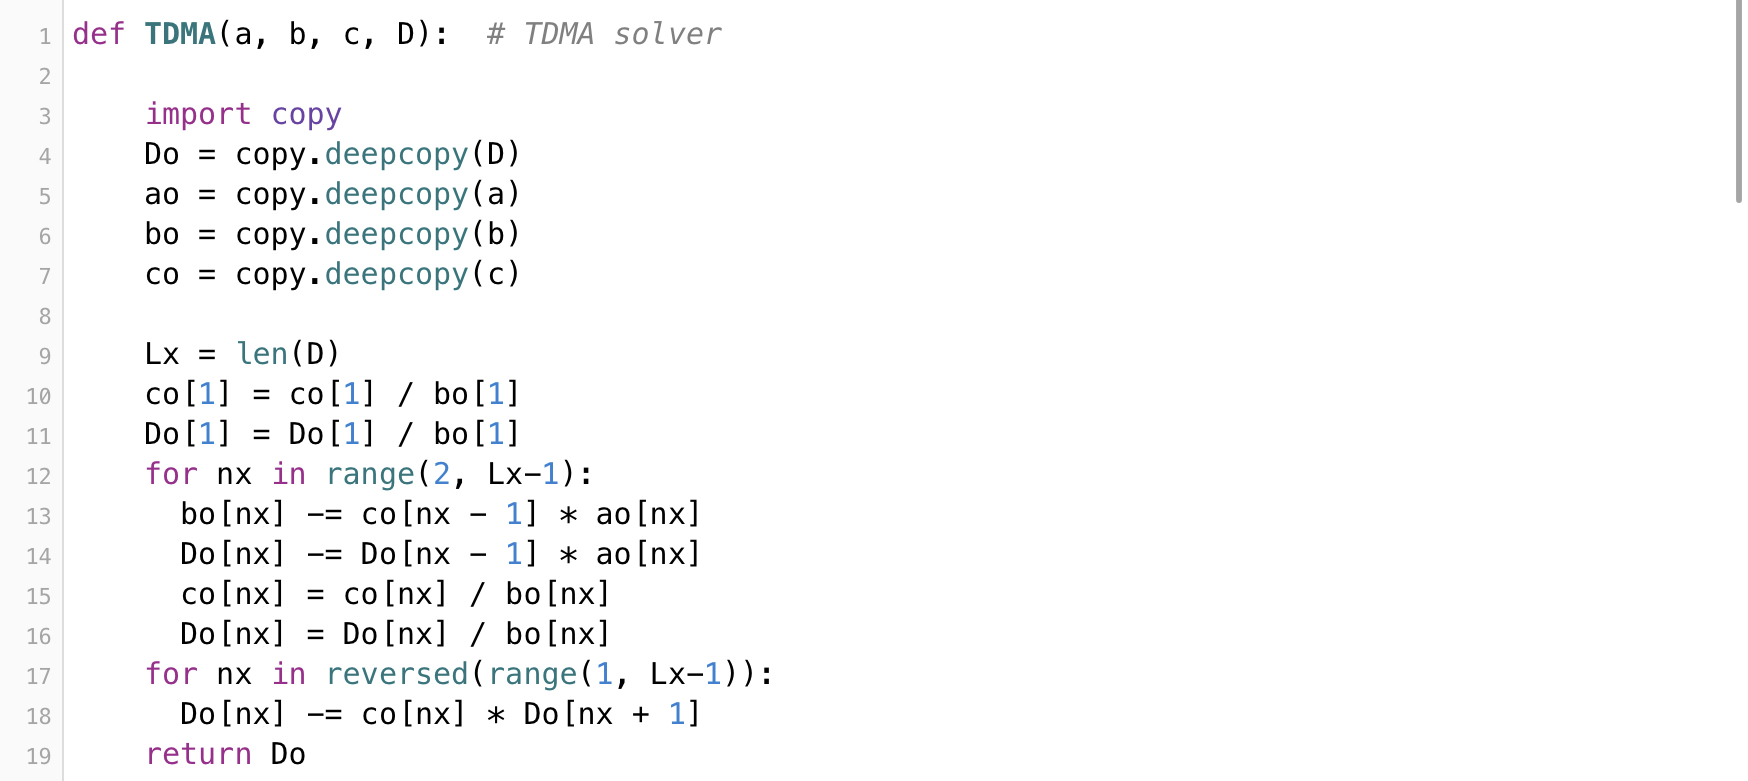
\includegraphics[scale=0.25]{TDMA solver.jpg} 
\caption{TDMA Solver code} 
\label{TDMA Solver code} 
\end{figure}


For backward Euler method and C-N method, we can notice their matrix A are different. Also, it is obvious that the C-N method also need us to first deal with matrix B. Thus, the Solver for Backward Euler and C-N are different. However, they can use same TDMA solver by input different a, b, c, d.\\


(The more detailed Algorithm is showing on Appendix page)


\subsection{Backward Euler Solver}
The Backward Euler Solver is showing below:


\begin{figure}[H] 
\centering 
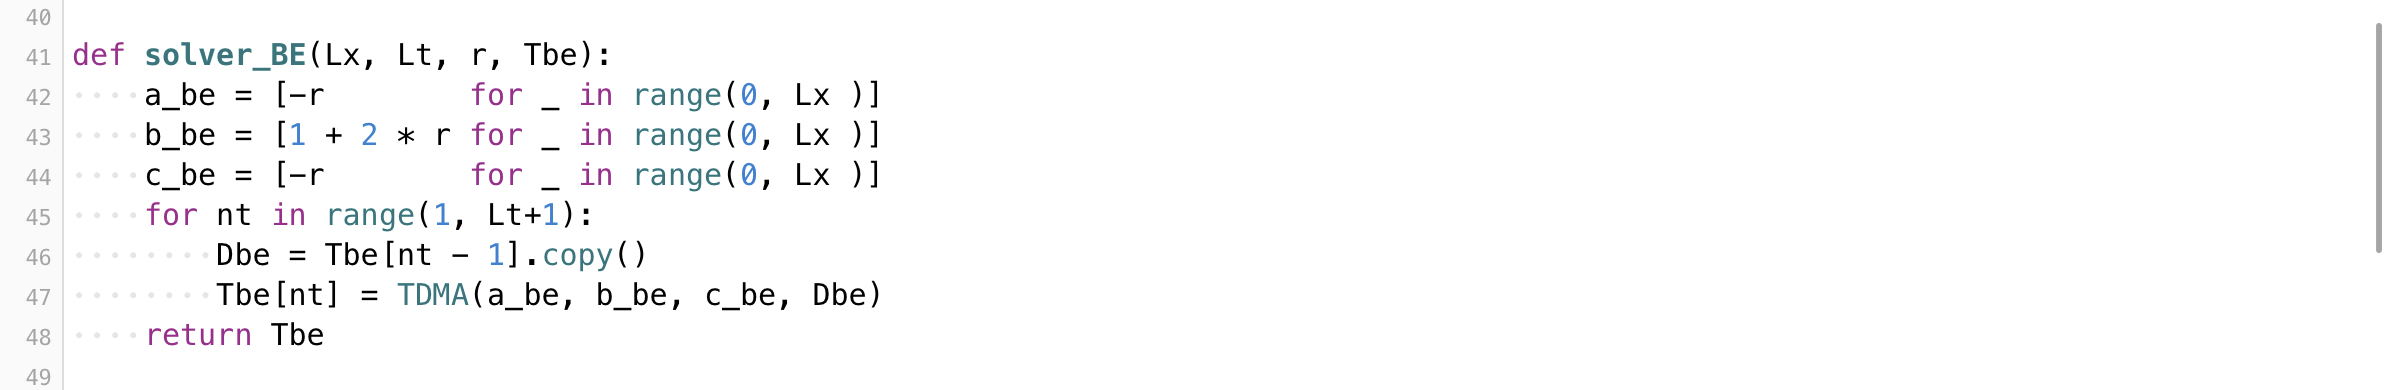
\includegraphics[scale=0.25]{Backward Euler Solver.jpg} 
\caption{Backward Euler Solver code} 
\label{TDMA Solver code} 
\end{figure}




\subsection{Crank-Nicolson Solver}


\begin{figure}[H] 
\centering 
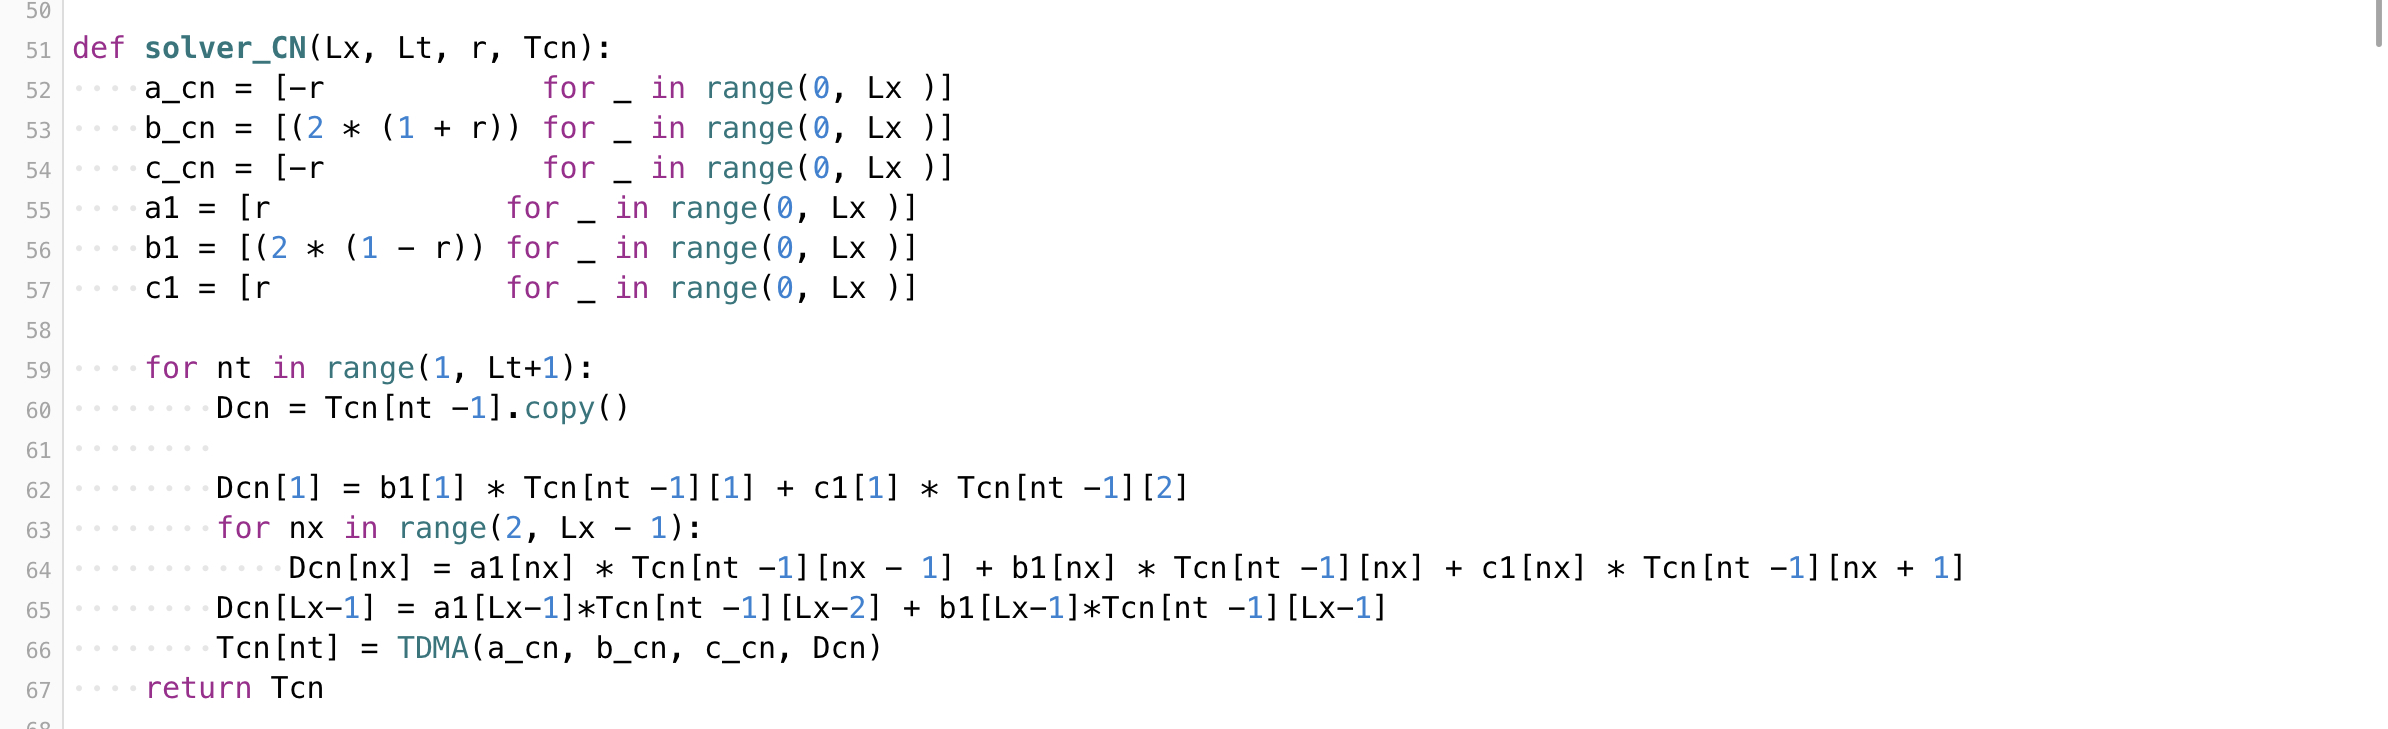
\includegraphics[scale=0.25]{C-N method Solver.jpg} 
\caption{C-N method Solver code} 
\label{TDMA Solver code} 
\end{figure}














%%%%%%%%%%%%%%%%%%%%%%%%%%%%%%%%%%%%%%%%

\section{(c) m=2, $\triangle x$=2$\pi$/20 and r=1/3}
\subsection{Plot Compare Numerical and Exact Solutions}
Apply Solvers for Forward Euler, Backward Euler, and Crank-Nicolson, and Exact Solution, the figures is showing below:





\begin{figure}[H] 
\centering 
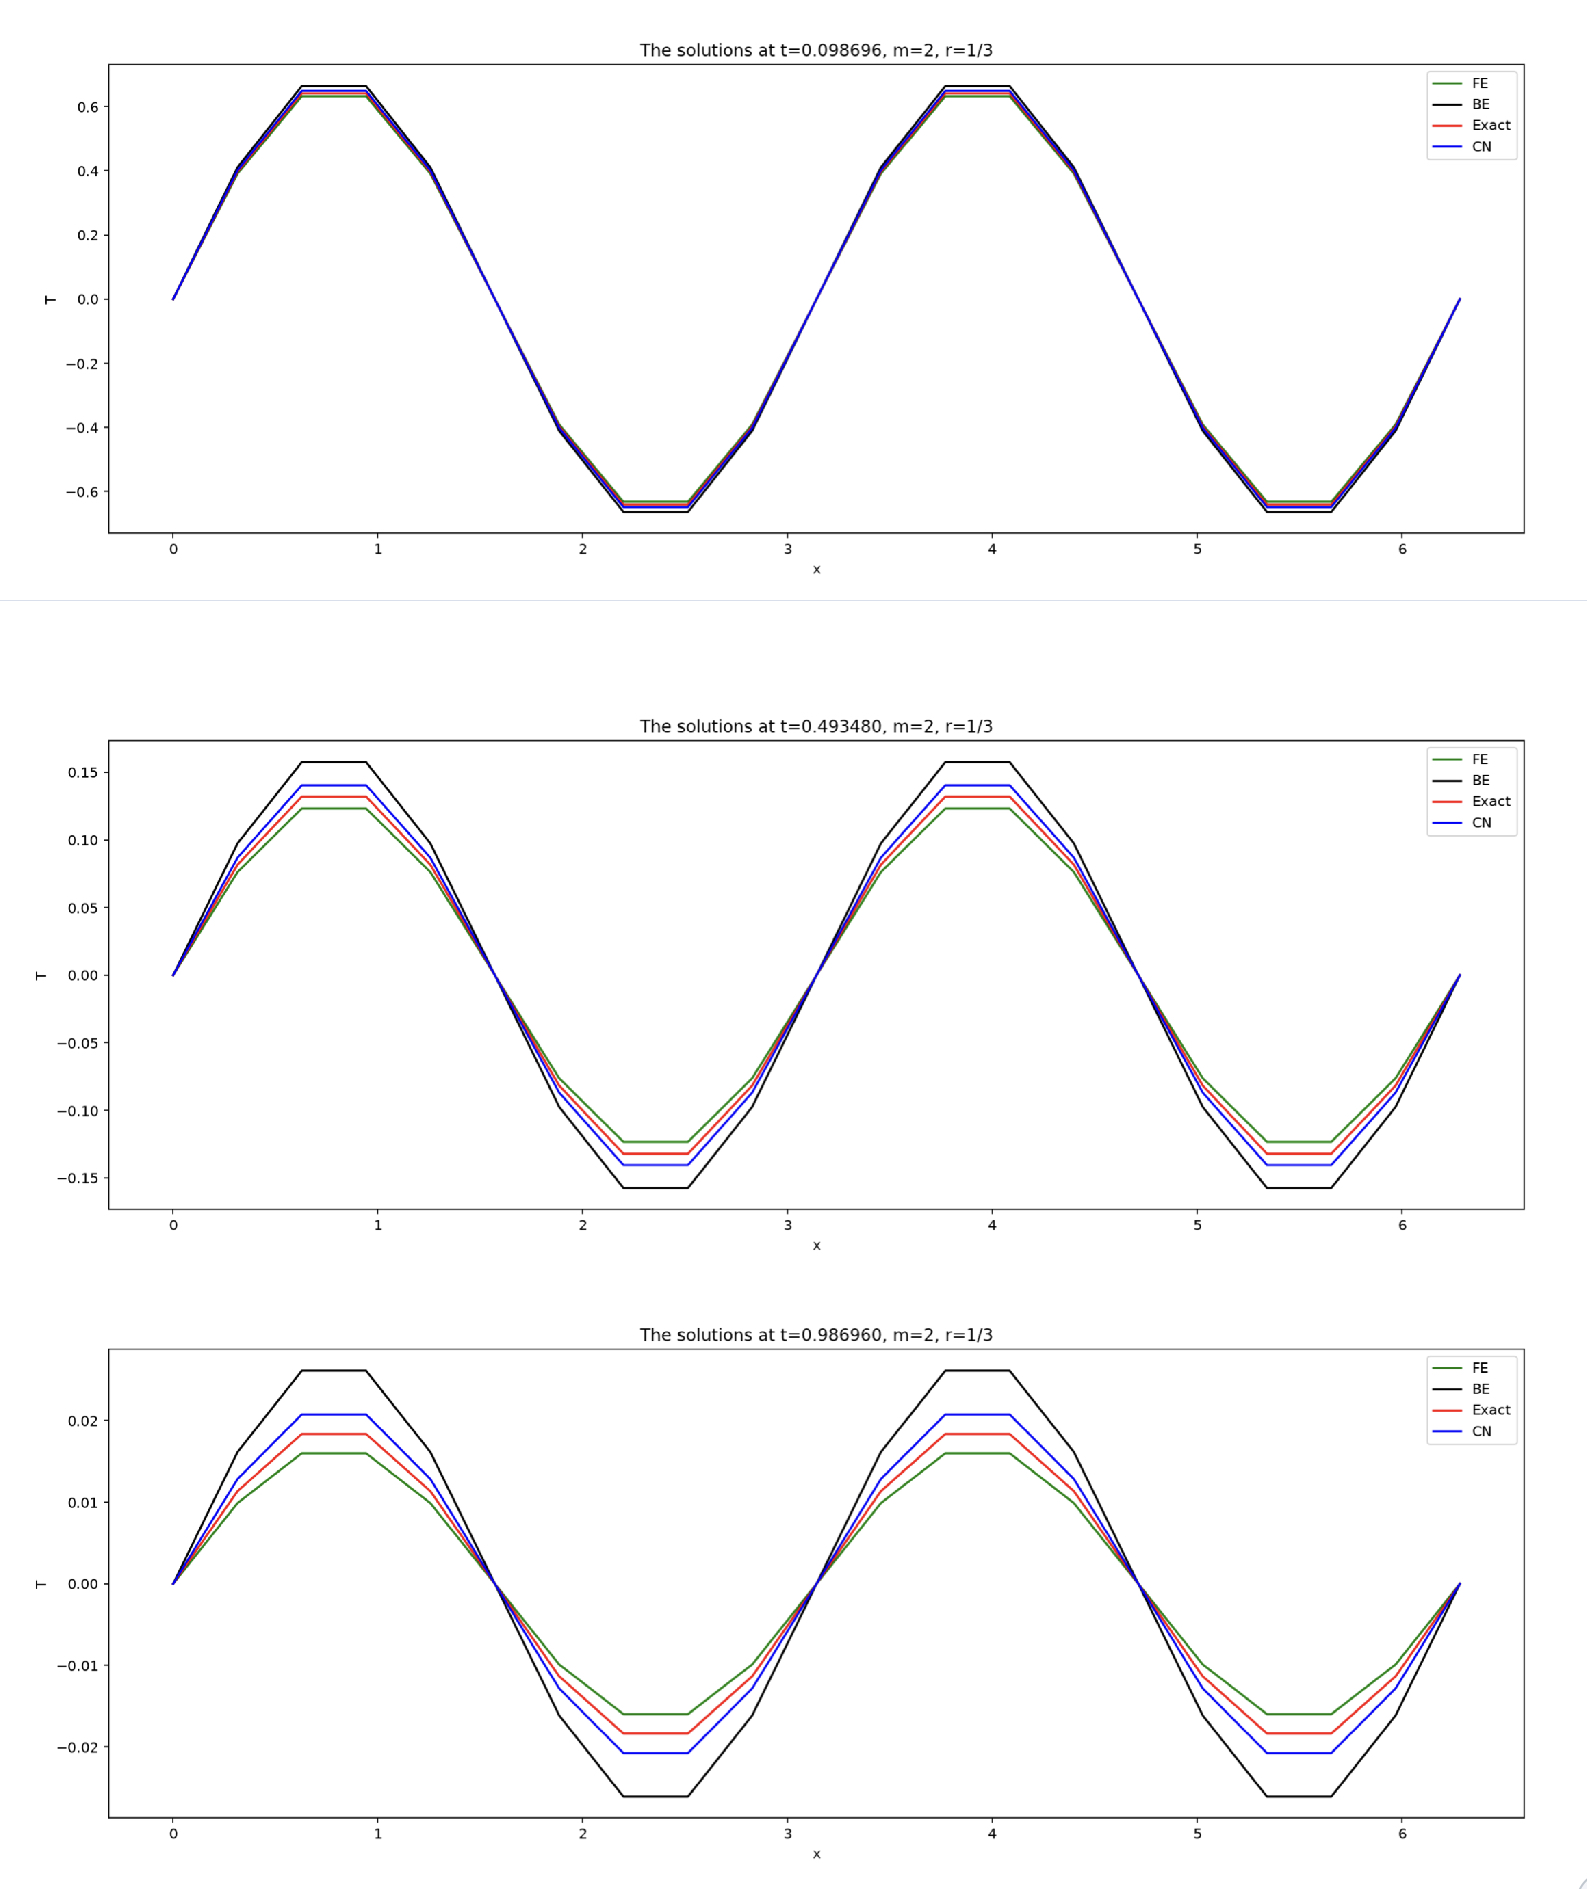
\includegraphics[scale=0.25]{figures for c.jpg} 
\caption{figures for different methods} 
\label{TDMA Solver code} 
\end{figure}



It shows during time, the error from numerical solutions to exact solution is getting bigger, while the Crank-Nicolson method and Forward Euler method is more closer to the exact solution than others.












\subsection{Errors and Characteristics}
\subsubsection{Error Scale}


\begin{figure}[H] 
\centering 
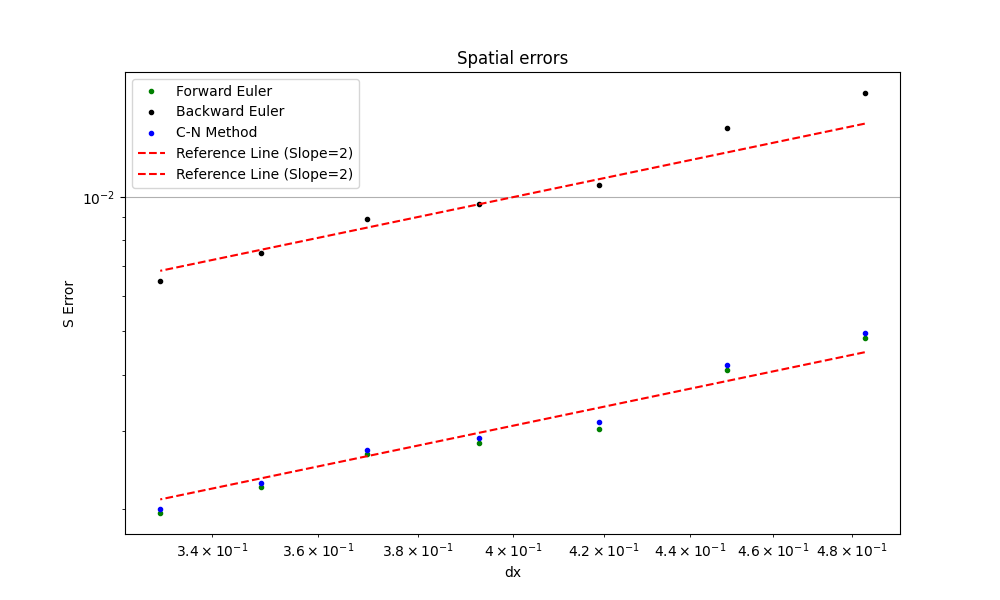
\includegraphics[scale=0.4]{Error growing.jpg} 
\caption{log-log plot for error increasing among dx} 
\label{TDMA Solver code} 
\end{figure}

The figure could show error growing is $O\left( \triangle x^{2}\right)  $, as its plot have slop 2





\subsubsection{VN stability analysis}

Among Von-Neumann stability analysis, the error could be express as $e^{ikx}$, while the exact solution is the numerical solution minus error, and the numerical solution fulfill the equation requirement, it turned out error fulfill our differential equation. Thus, the error of different methods could be shown, as the absolute value of error amplification should never greater than 1, the VN stability analysis shows its registration for different methods:\\

For the Forward Euler method, is:

$$ \left\vert 1+2r\left( cos\left( \beta_{k} \right)  -1\right)  \right\vert <1 $$

For Backward Euler method, is:

$$\left\vert \begin{bmatrix}1+2r\left( 1-cos\left( \beta_{k} \right)  \right)  \end{bmatrix}^{-1} \right\vert  <1$$\\



For Crank-Nicolson method, is:

$$ \left\vert  \frac{1-r\left( 1-cos\left( \beta_{k} \right)  \right)  }{1+r\left( 1-cos\left( \beta_{k} \right)  \right) }\right\vert  <1 $$\\




It could be seen for both Backward Euler and Crank-Nicolson method, the Von-Neumann Stability limit is always fulfilled, that its implicit method's unconditionally stable characterization.\\

For Forward Euler method, it turns out to full fill Von-Neumann Stability limit , $r \leqslant \frac{1}{2} $ is its requirement.




\subsubsection{If r $>$ 1/2 }


If r is larger than 1/2, we known it won't influence implicit scheme, only different is Forward Euler method.


\begin{figure}[H] 
\centering 
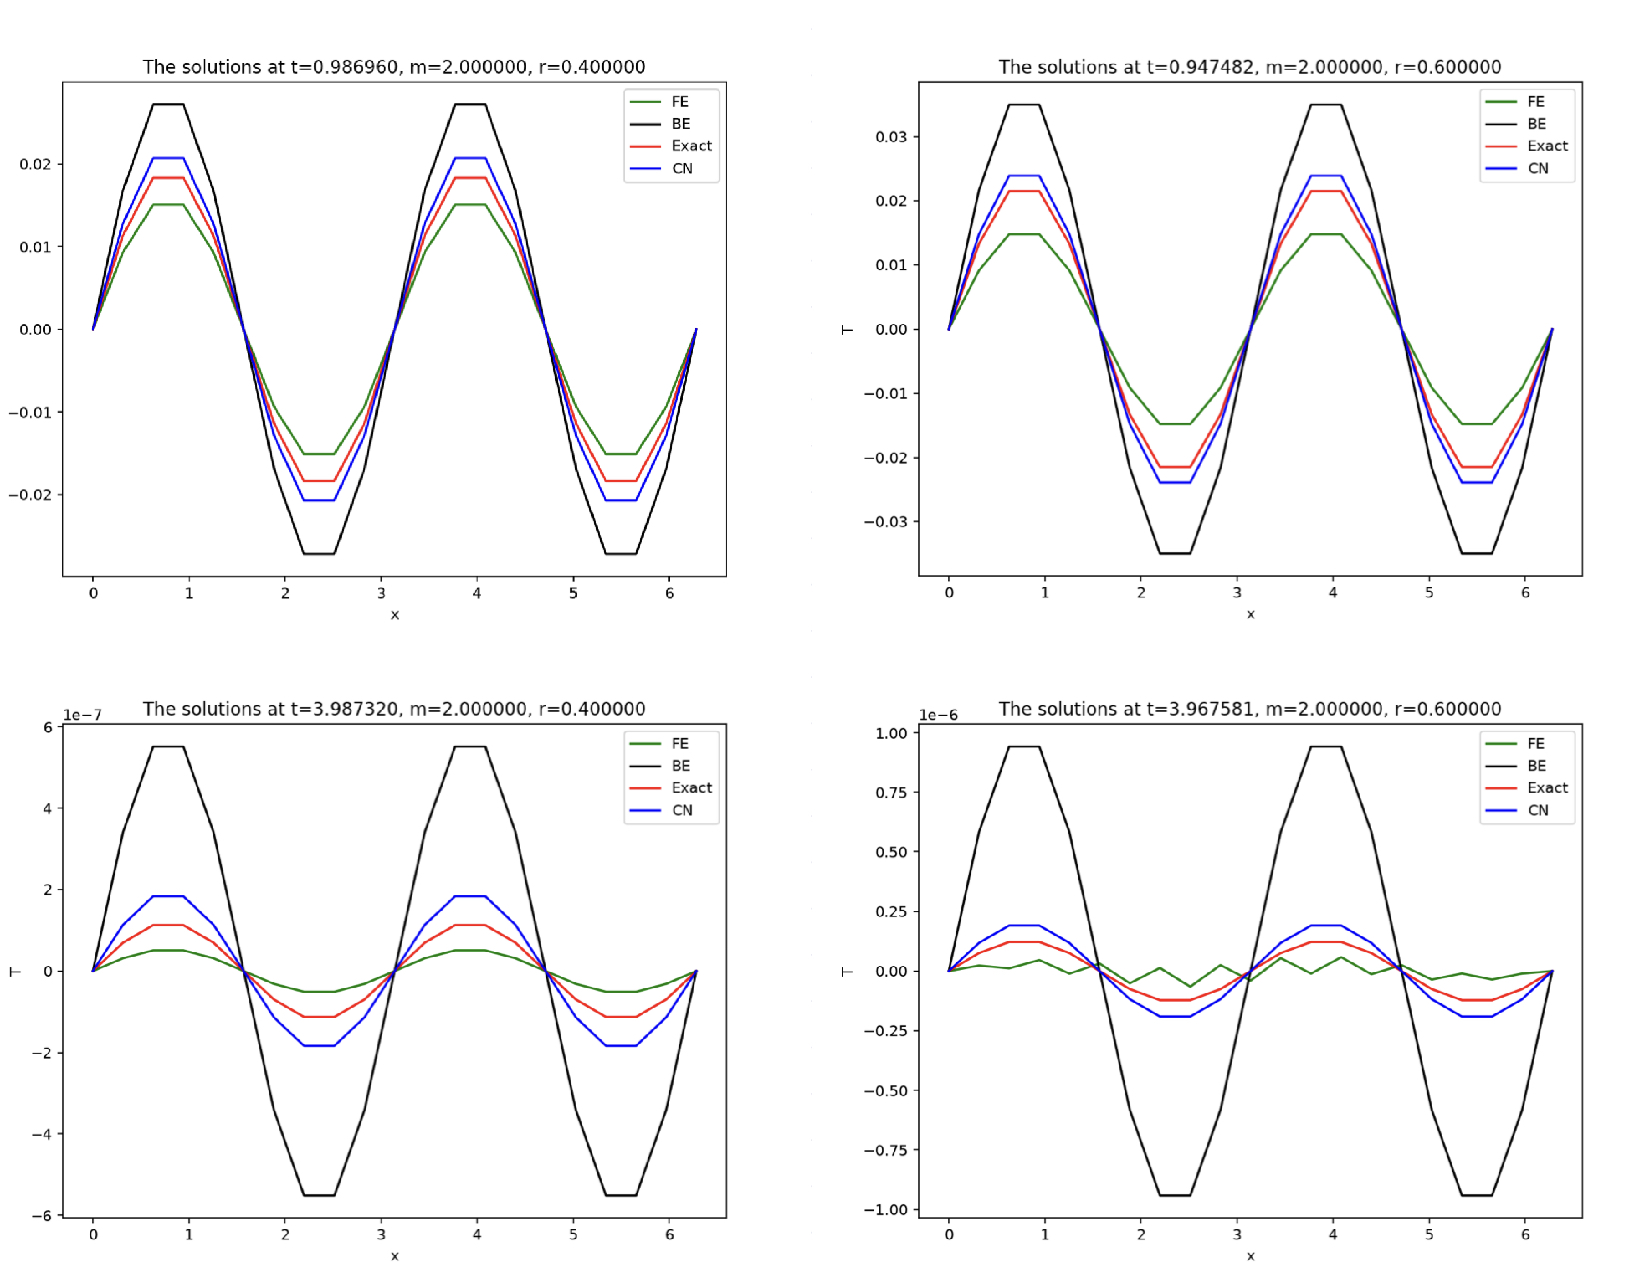
\includegraphics[scale=0.3]{r too large.jpg} 
\caption{left part is r=0.4, right part is r=0.6} 
\label{TDMA Solver code} 
\end{figure}

For the lower right figure, it is obvious that the Forward Euler method, the solution becomes unstable.



\begin{figure}[H] 
\centering 
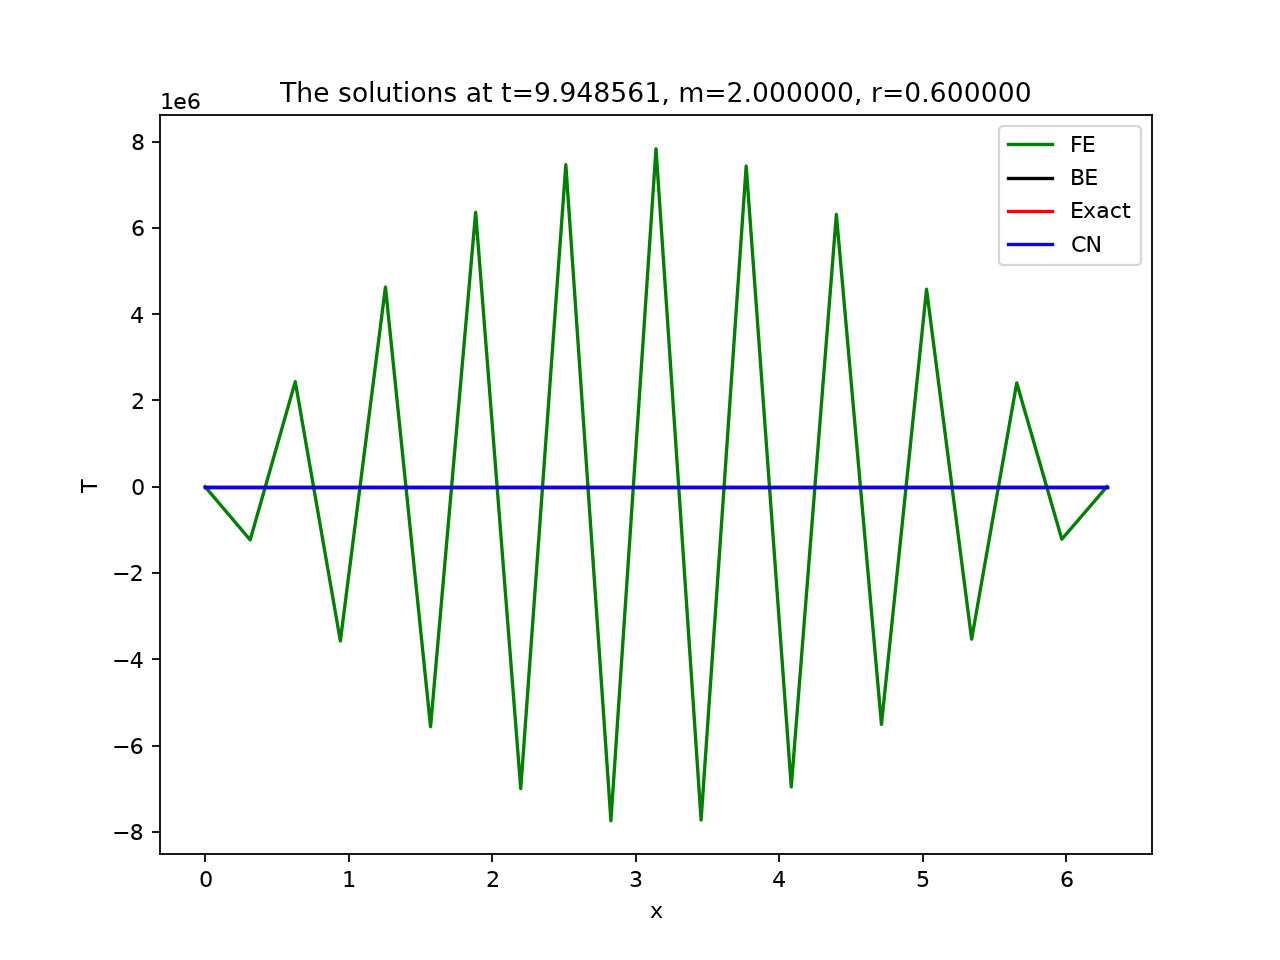
\includegraphics[scale=0.25]{Unstable FE.jpg} 
\caption{t=10,r=0.6, clearly unstable for Forward Euler} 
\label{TDMA Solver code} 
\end{figure}














%%%%%%%%%%%%%%%%%%%%%%%%%%%%%%%%%%%
\section{(d) $\triangle x$=2$\pi$/20 and r=0.5, and for m=3, 5, and 7.}
\subsection{The Plot}

\subsubsection{The Solutions at  t=0.5s}
For time = 0.5s, the solutions are showing below:

\begin{figure}[H] 
\centering 
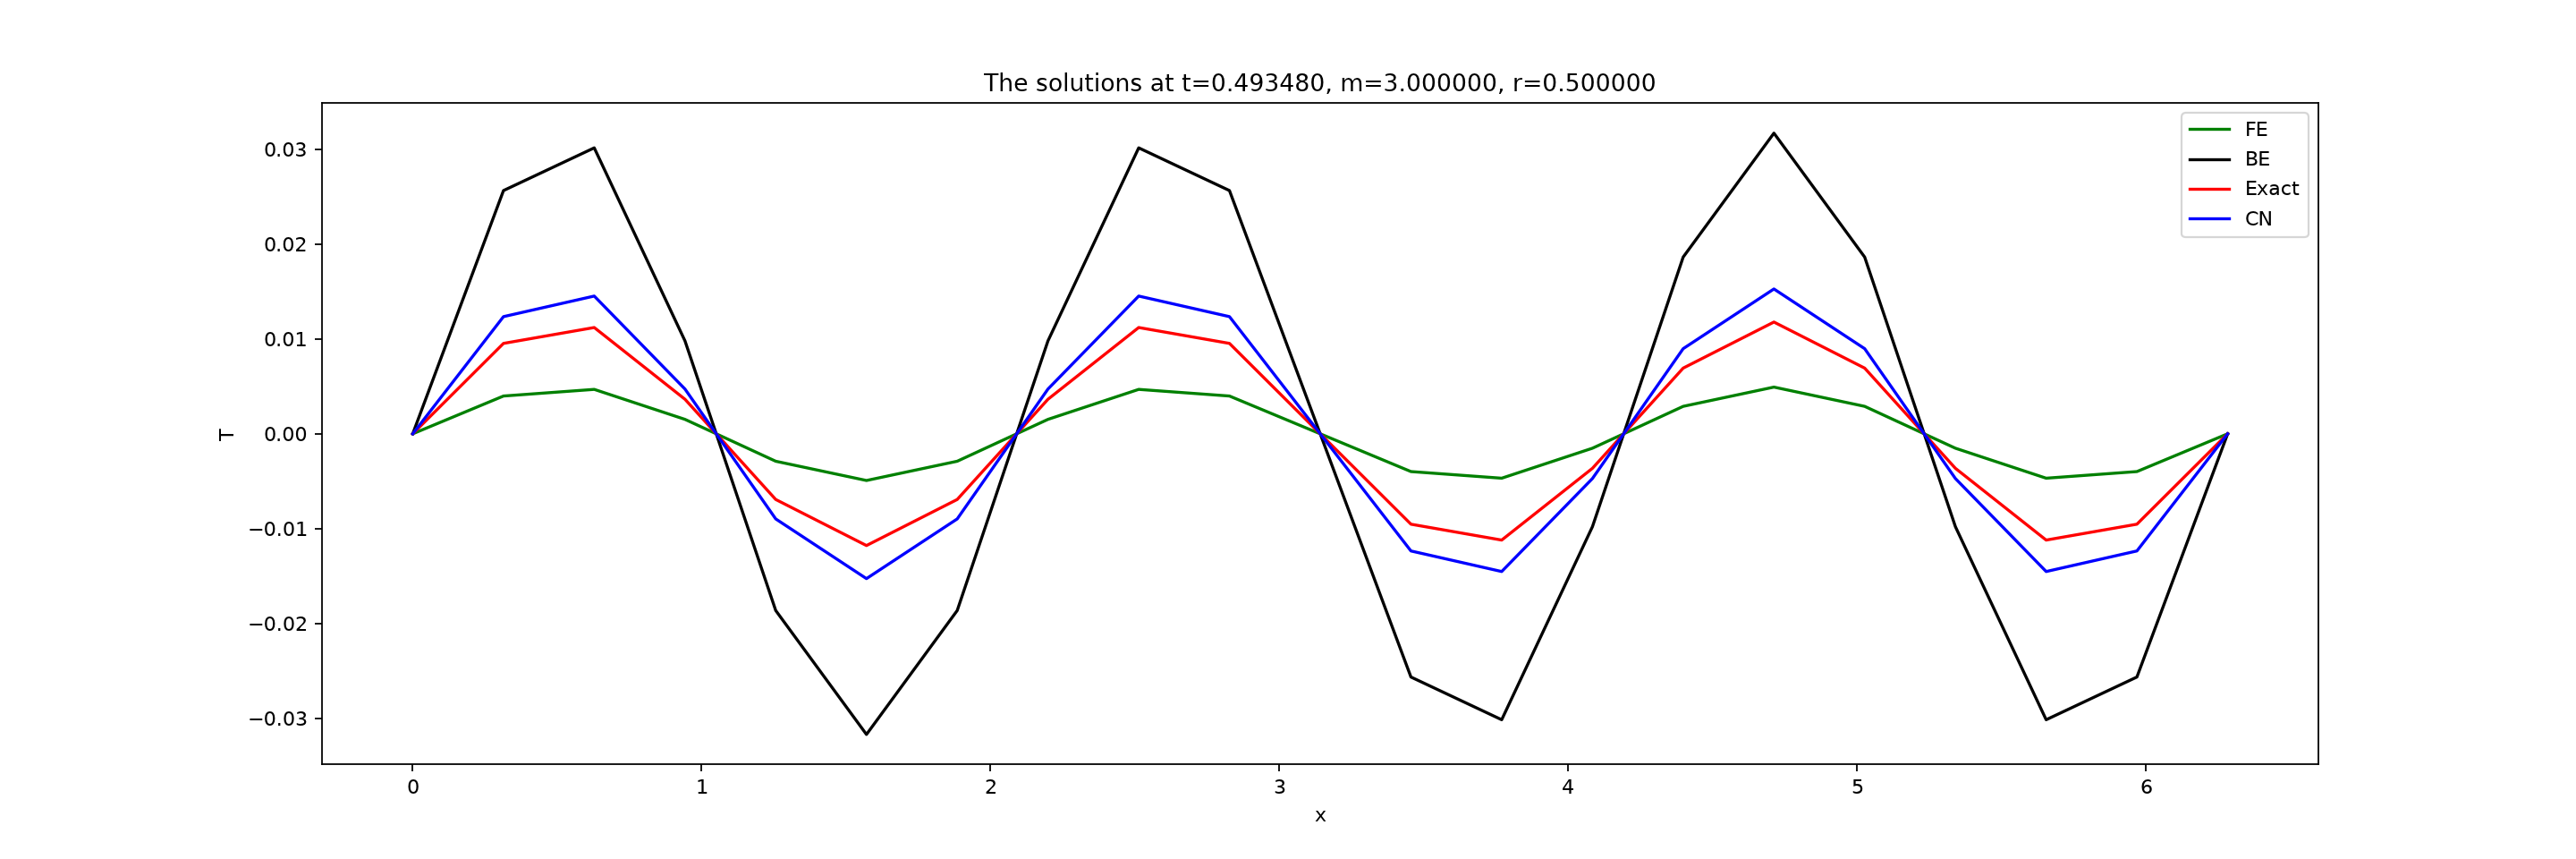
\includegraphics[scale=0.15]{0.5,0.3,0.5.jpg} 
\caption{t = 0.5, m =3, r = 0.5} 
\label{TDMA Solver code} 
\end{figure}

It can be seen on this situation, Backward Euler and Forward Euler have the low accuracy, while C-N method is most close to exact solution.


\begin{figure}[H] 
\centering 
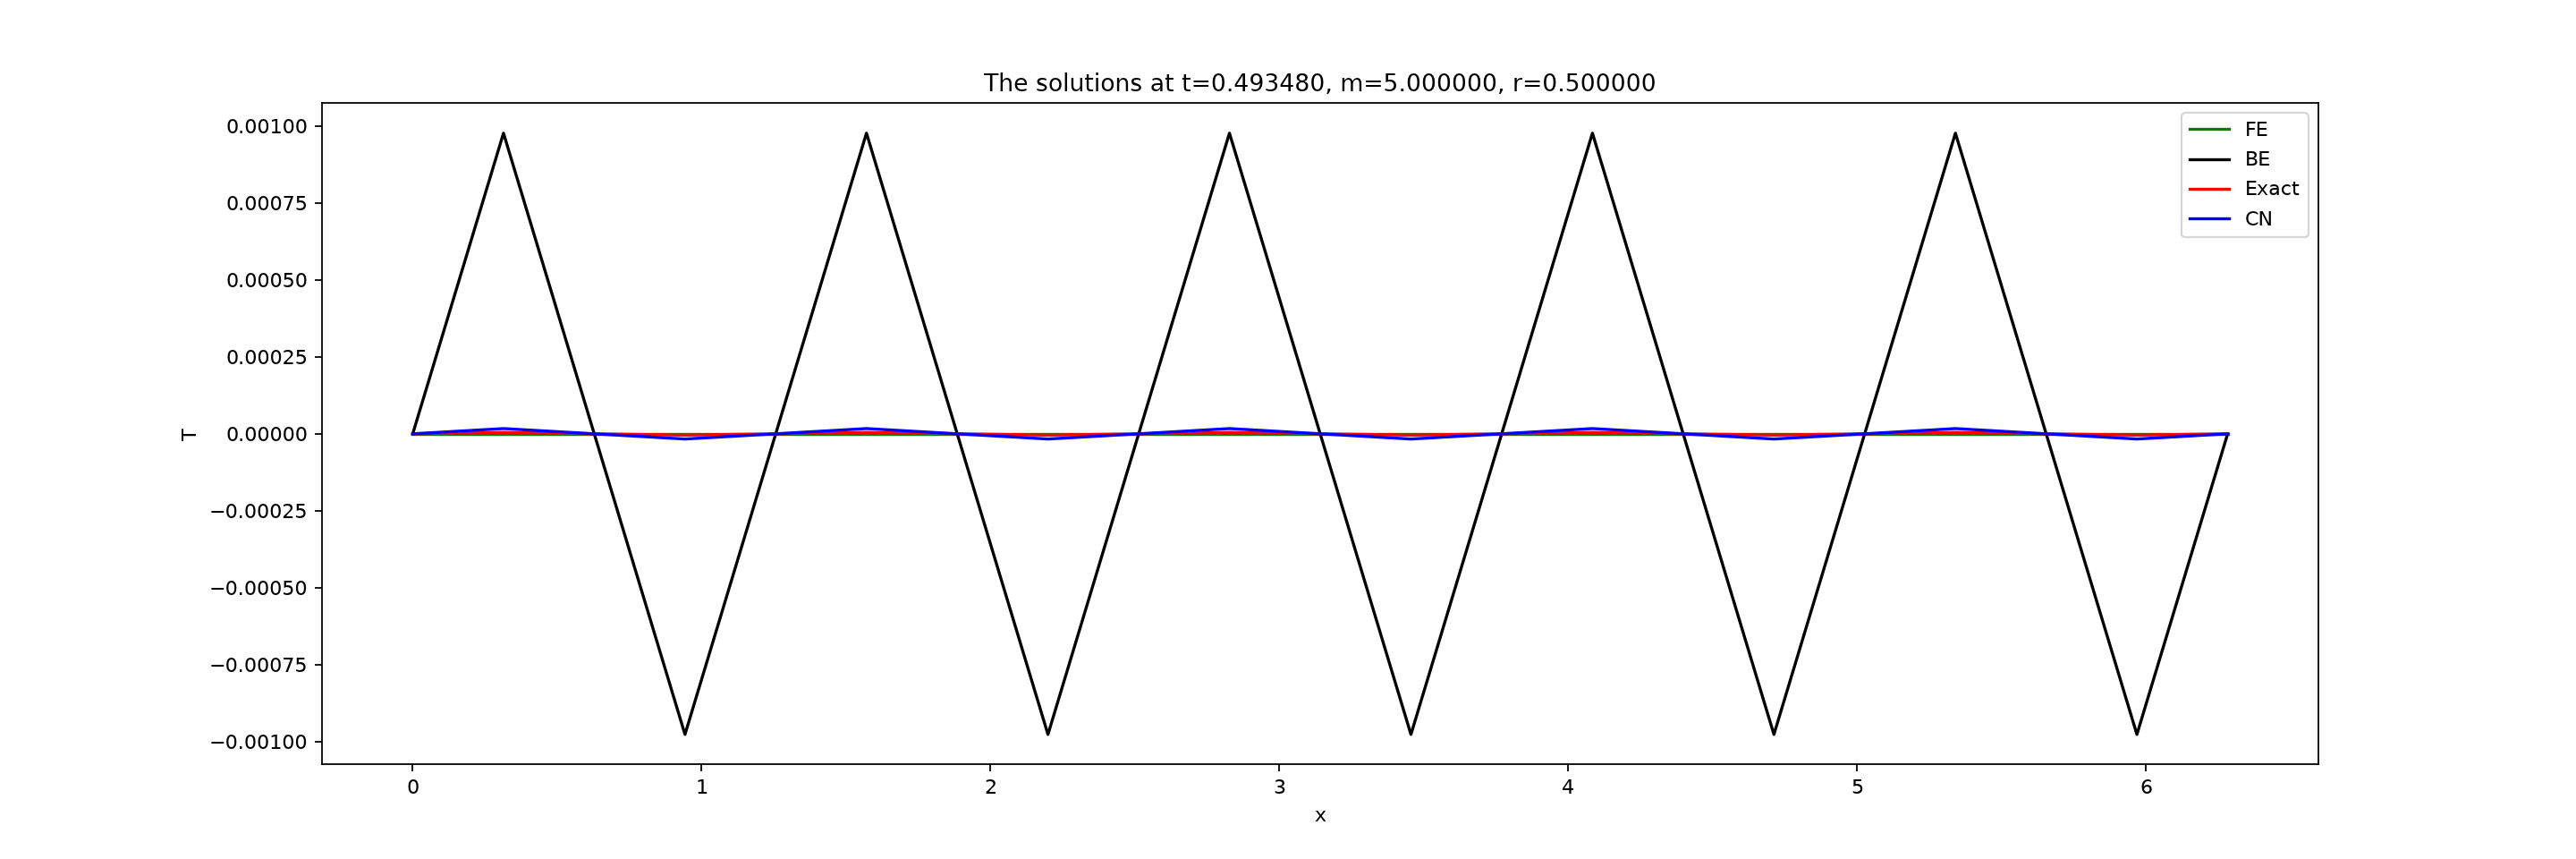
\includegraphics[scale=0.15]{0.5,0.5,0.5.jpg} 
\caption{t = 0.5, m =5, r = 0.5} 
\label{TDMA Solver code} 
\end{figure}

It can be seen on this situation, Backward Euler have the lowest accuracy.

\begin{figure}[H] 
\centering 
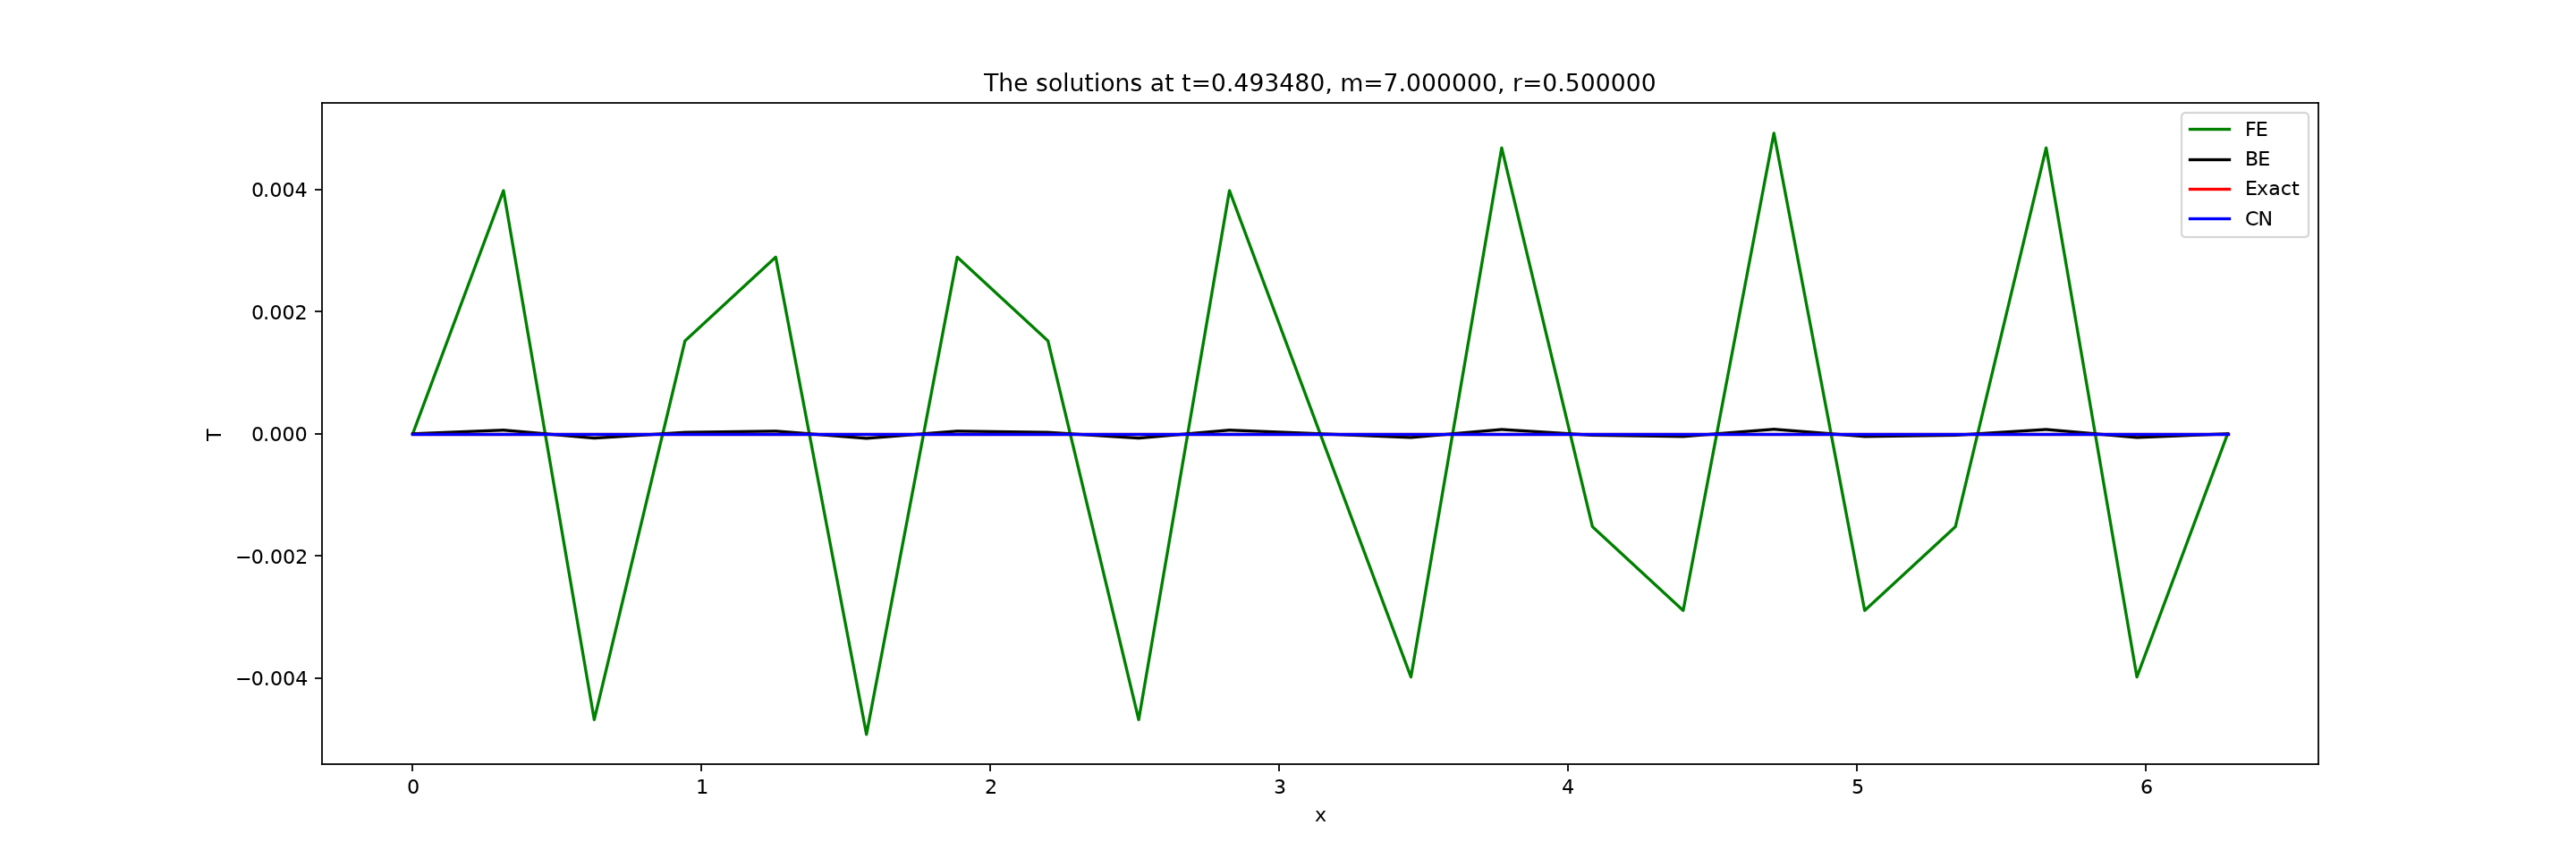
\includegraphics[scale=0.15]{0.5,0.7,0.5.jpg} 
\caption{t = 0.5, m =7, r = 0.5} 
\label{TDMA Solver code} 
\end{figure}

It can be seen on this situation, Forward Euler turns out have the lowest accuracy, while C-N method is still most accurate to exact solution.







\subsubsection{The numerical solutions at t=0.5s compare to t=0.1s}
Compare t=0.5 to t=0.1, the plots is showing below:


\begin{figure}[H] 
\centering 
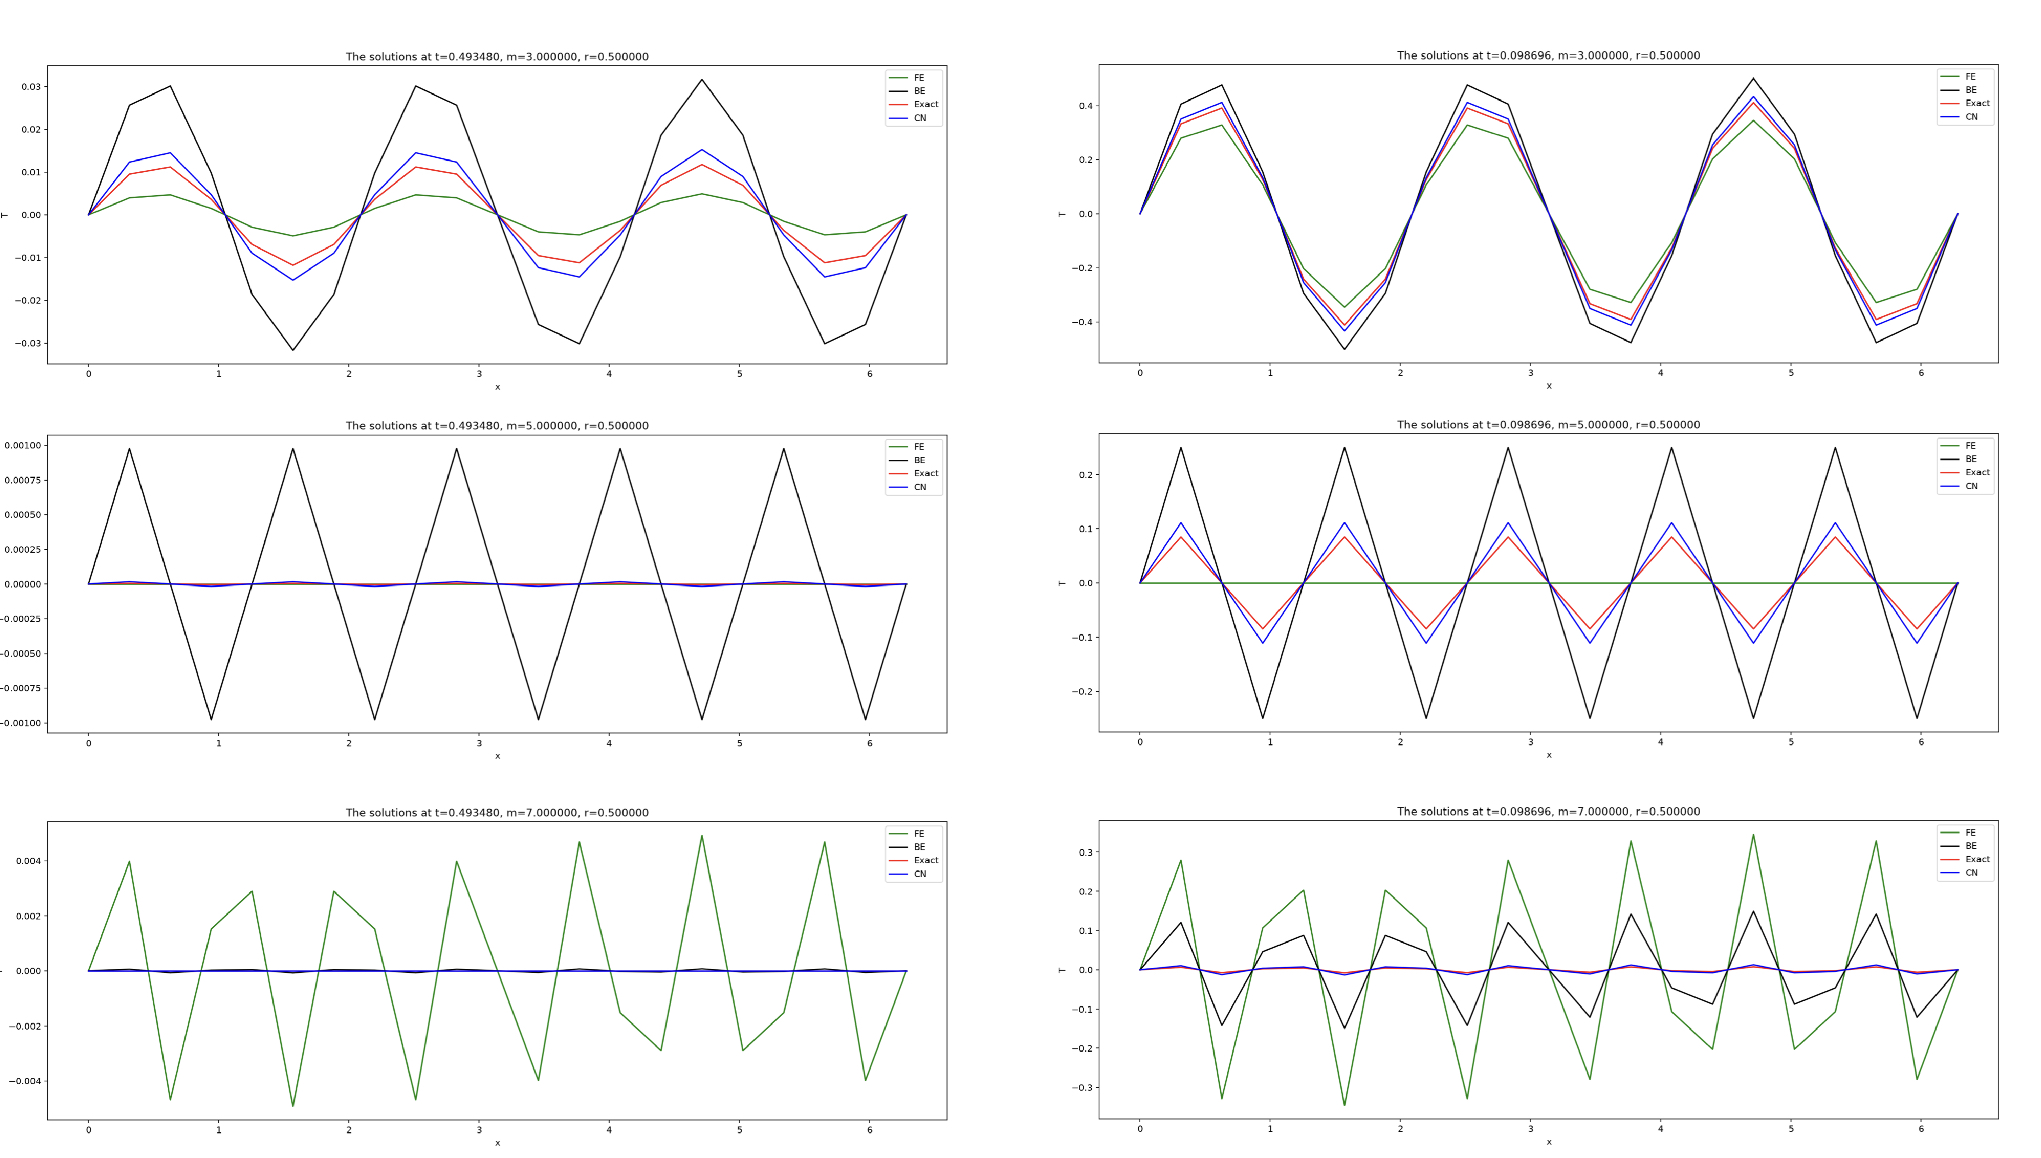
\includegraphics[scale=0.25]{figures for different methods.jpg} 
\caption{Comparison of t=0.5 and t=0.1} 
\label{TDMA Solver code} 
\end{figure}


It is clear that the C-N methods is most close to the exact solution, Backward Euler is the most inaccurate numerical solution for m=3 and m=5, and Forward Euler solution almost blow up at m=7, r = 0.5.\\

The comparison of t=0.5 and t=0.1 is showing much more clear that the solution we explained above.



\subsection{Amplification factor Analysis}


For exact solution, the Amplification factor G is showing below:
$$G^{e}_{k}=e^{-r\beta^{2}_{k} }$$

For the Forward Euler method, G is:

$$G_{k}=1+2r\left( cos\left( \beta_{k} \right)  -1\right)  $$

For Backward Euler method, G is:

$$G_{k}=\begin{bmatrix}1+2r\left( 1-cos\left( \beta_{k} \right)  \right)  \end{bmatrix}^{-1} $$



For Crank-Nicolson method, G is:

$$G_{k}=\frac{1-r\left( 1-cos\left( \beta_{k} \right)  \right)  }{1+r\left( 1-cos\left( \beta_{k} \right)  \right)  } $$


While r=0.5, m=3/5/7, the Amp number G for each situation can be showing below:

\begin{center}

\setlength{\tabcolsep}{10mm}{
\begin{tabular}{c | c c c}

\toprule
m & 3& 5 & 7\\
\toprule
$\beta_{k}$ & 0.94 & 1.57 & 2.19\\
\toprule
G(EX) & 0.64138 &  0.29121 & 0.08909\\
\midrule
G(FE) & 0.58778 &  1.11022e-16 & -0.58778\\
\midrule
G(BE) & 0.70811 &  0.50000 & 0.38643\\
\midrule
G(CN) & 0.65822 & 0.33333 & 0.11489\\
\bottomrule
\end{tabular}}
\end{center}


Could be seen at m=3, Bk=0.94, showing in the table and the first line of the plot, Amplification Factor from Max to Min is G(BE) \textgreater G(CN) \textgreater G(EX) \textgreater G(FE), where CN is most close to the Exact solution.\\


\begin{figure}[H] 
\centering 
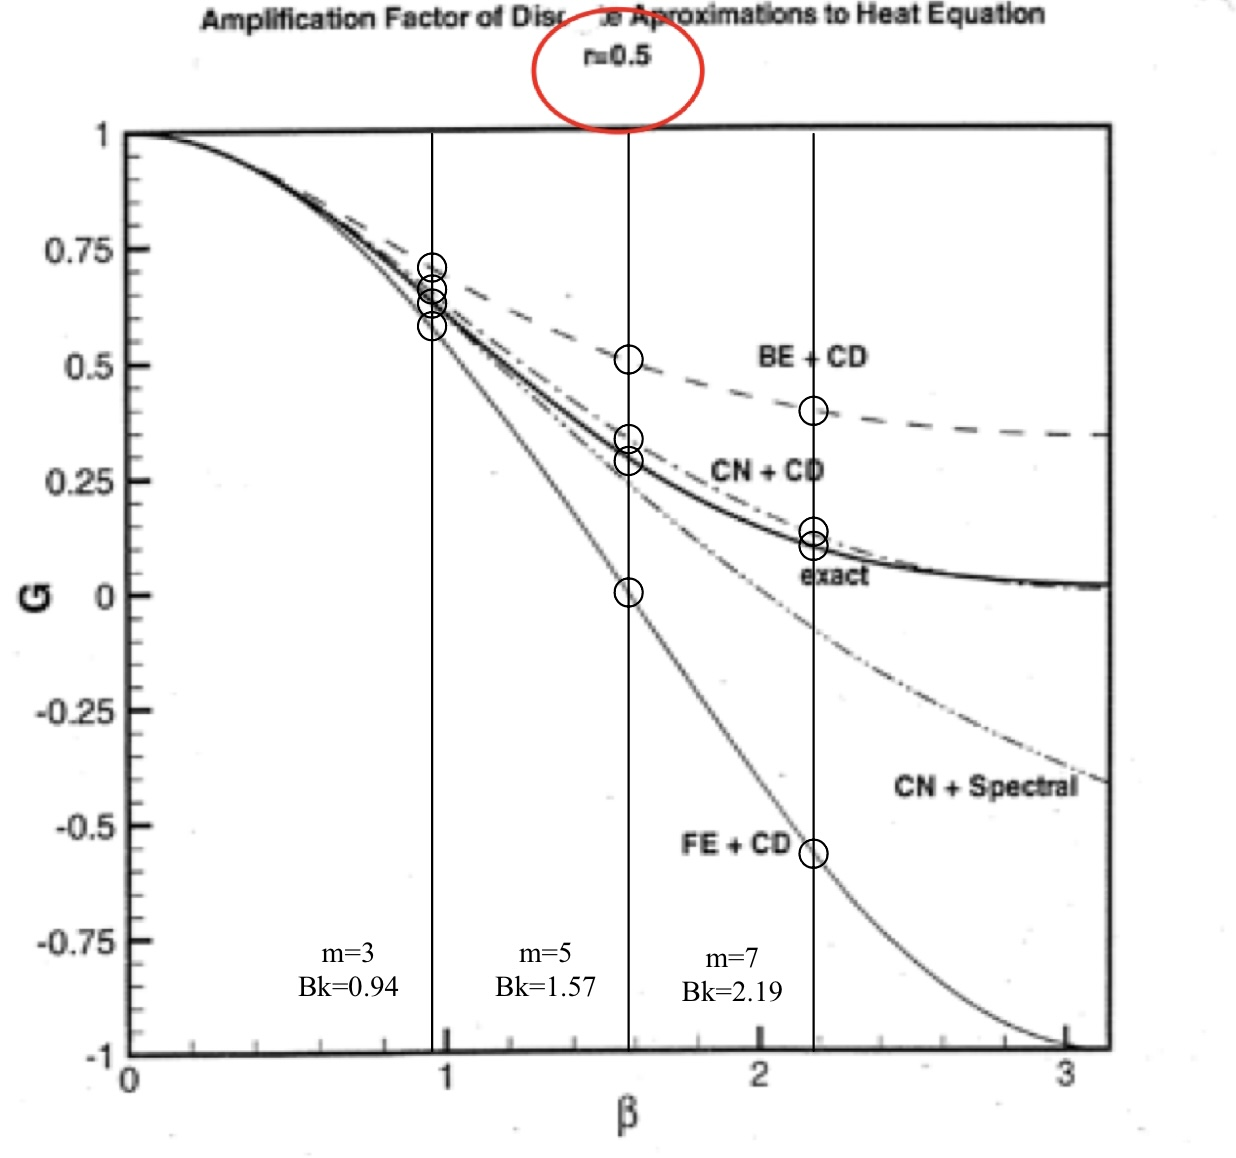
\includegraphics[scale=0.6]{Amp Figure.jpg} 
\caption{Amp Figure for EX, FE, BE, CN} 
\label{TDMA Solver code} 
\end{figure}





We also can notice at m=5, Bk=1.57, showing in the table and the second line of the plot, Amplification Factor from Max to Min is still  BE,CN,EX,FE, where CN is most close to the Exact solution, though the difference between numerical solutions and Exact solutions of Amplification Number is much larger than m=3. Also need to notice that in this case, Amplification Number of Forward Euler is pretty close to 0, where is also shown in the solution pictures before.\\




At m=7, Bk=2.19, showing in the table and the third line of the plot, Amplification Factor from Max to Min is still BE,CN,EX,FE, where CN is most close to the Exact solution, also need to notice at this case, FE Forward Euler method’s Amp Number is smaller than 0.



\section{Appendix}
\subsection{Exact Solution}


\begin{figure}[H] 
\centering 
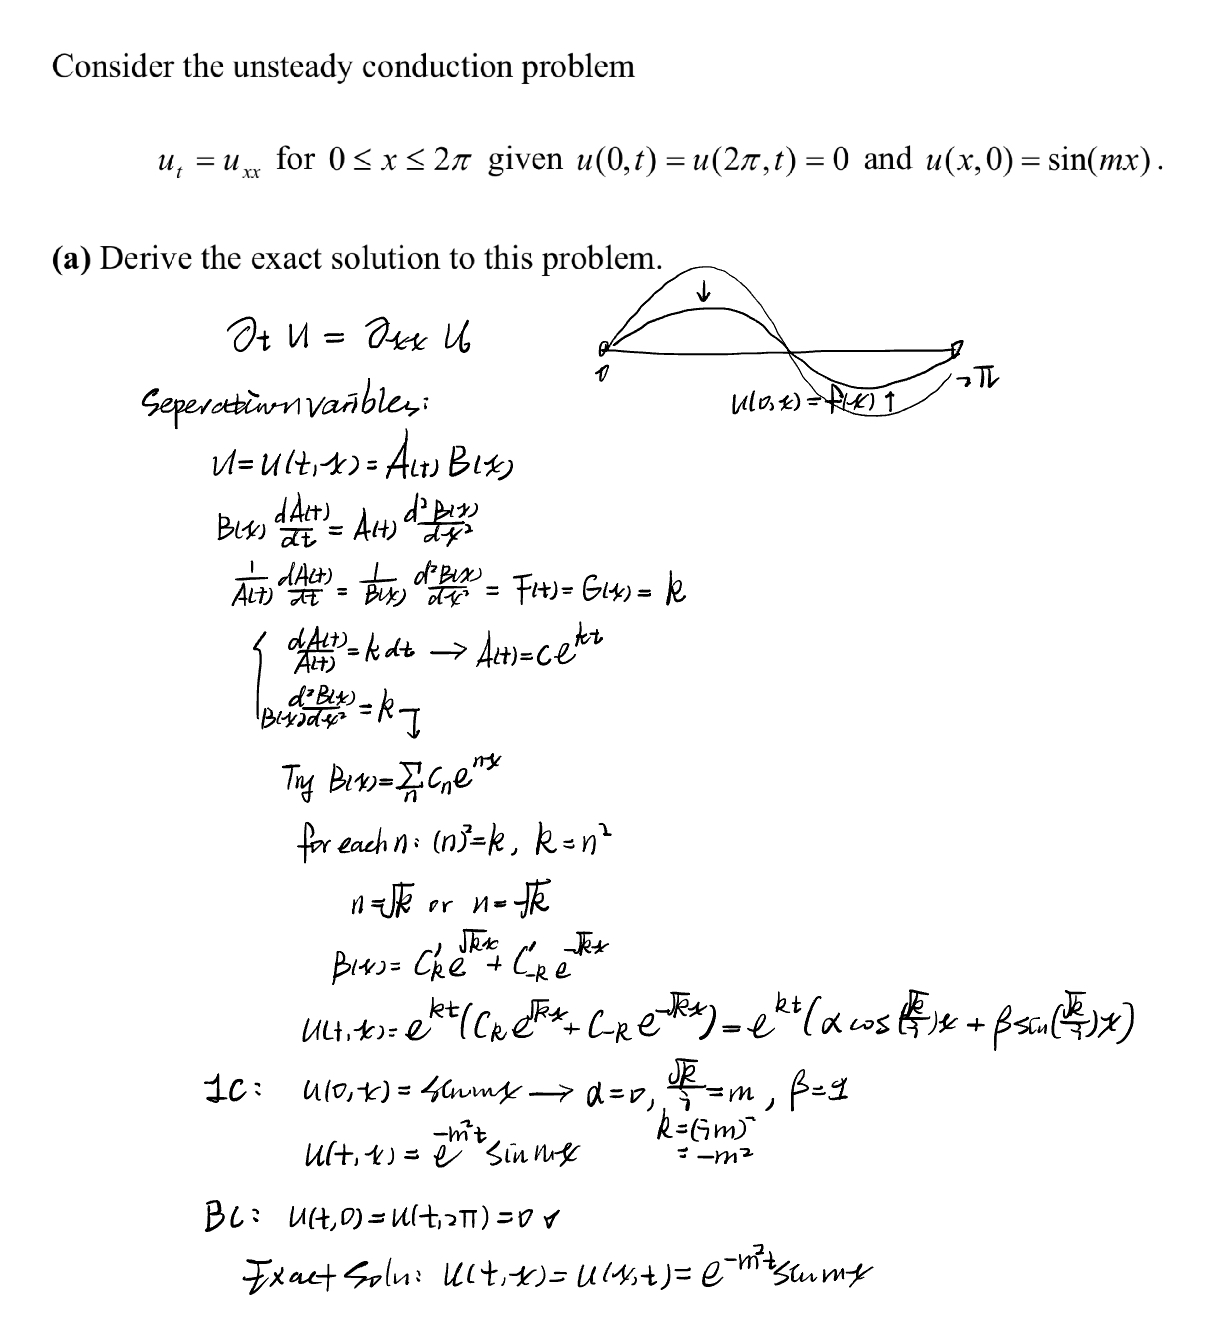
\includegraphics[scale=0.4]{exact solution.jpg} 
\label{TDMA Solver code} 
\end{figure}




\subsection{Backward Euler and C-N Scheme}
\begin{figure}[H] 
\centering 
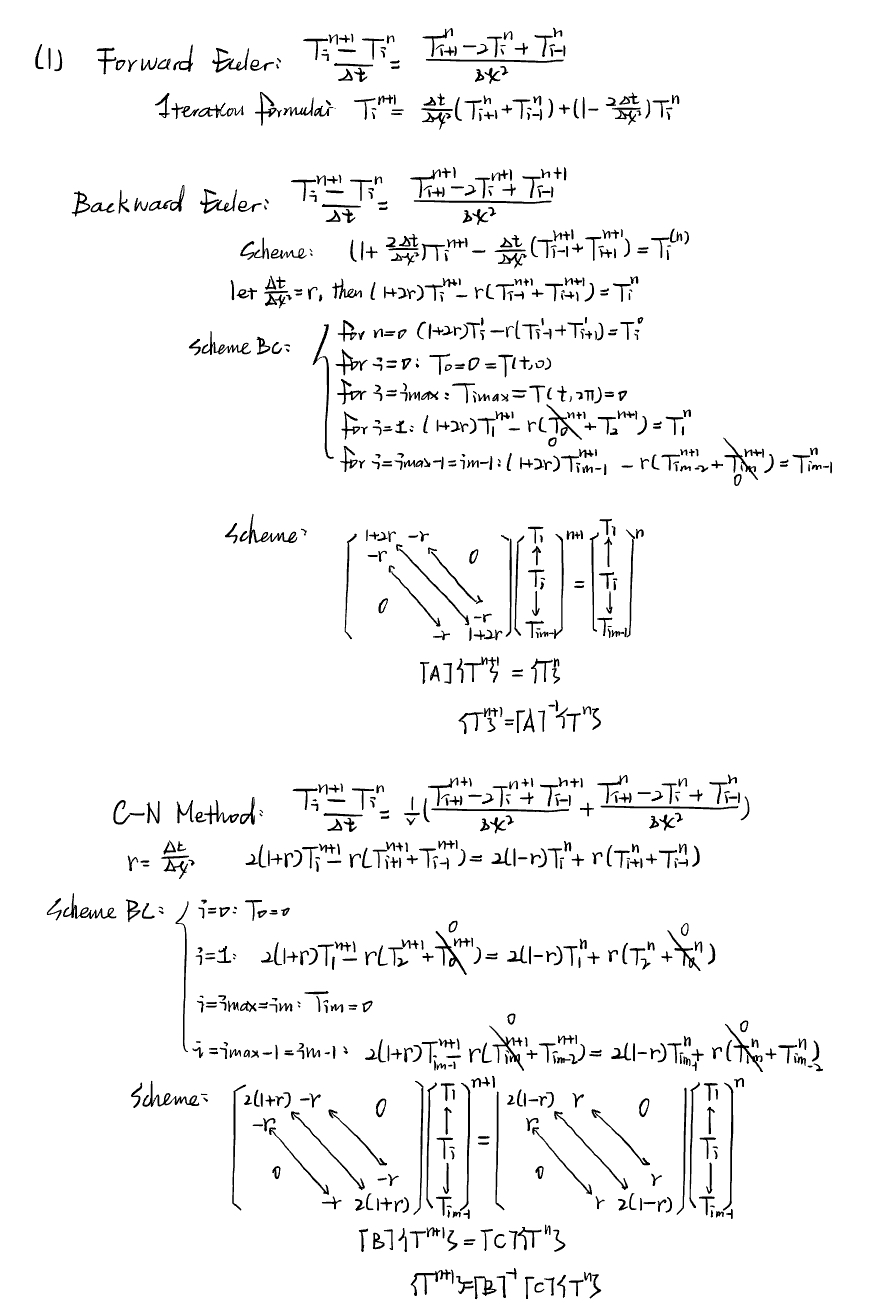
\includegraphics[scale=0.5]{Schemes.jpg} 
\end{figure}




\subsection{Gauss Elimination}
\begin{figure}[H] 
\centering 
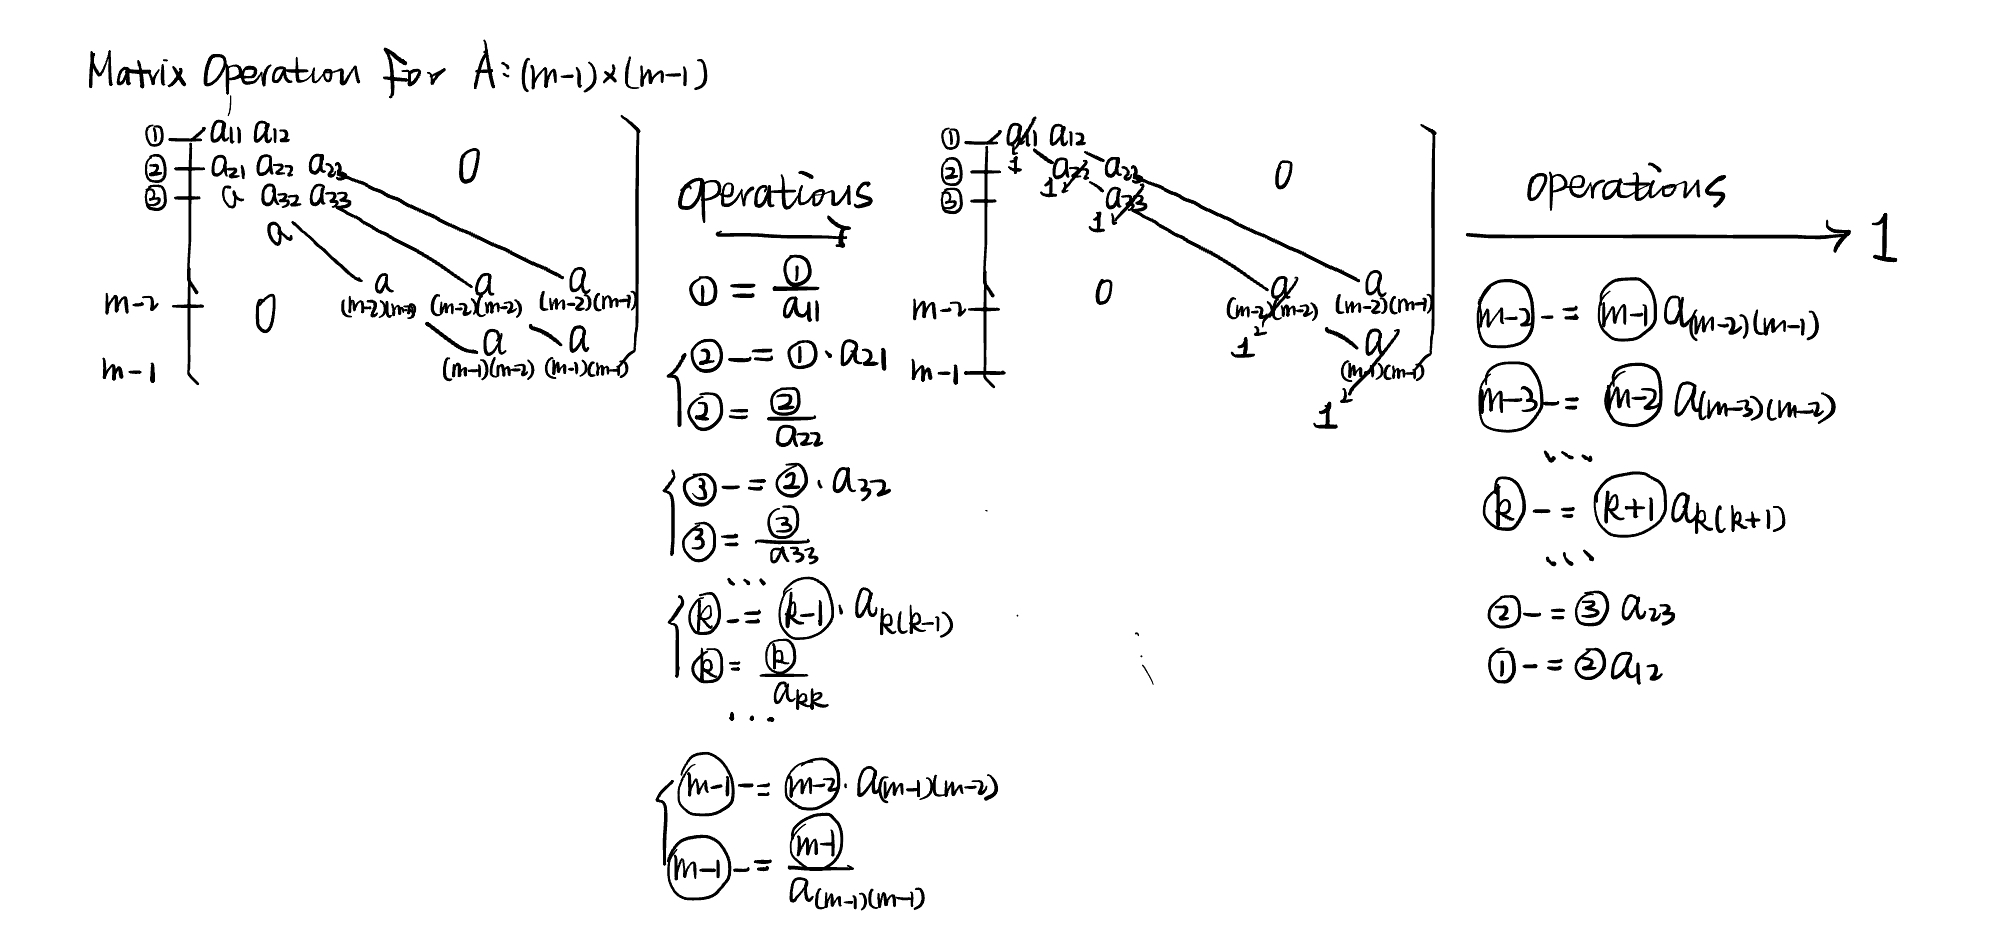
\includegraphics[scale=0.2]{Gauss Elimination.jpg} 
\end{figure}


\subsection{Solver Algorithm}
\begin{figure}[H] 
\centering 
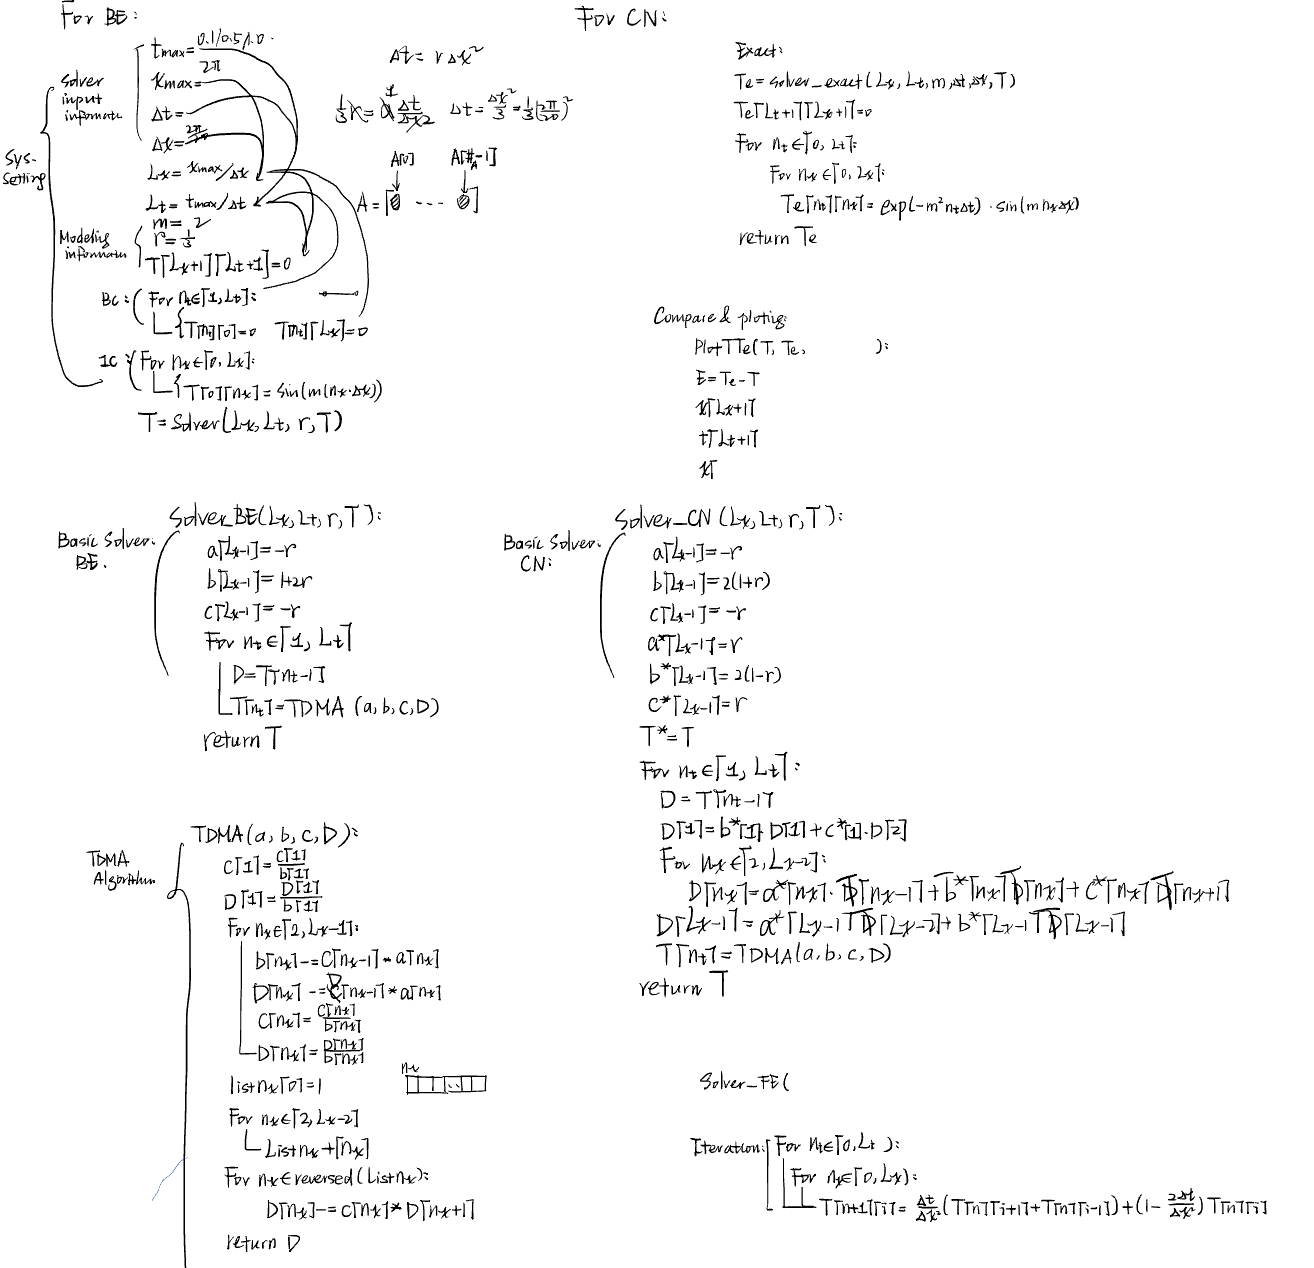
\includegraphics[scale=0.3]{Solver Algorithm.jpg} 
\end{figure}




























\end{document}
\end